%----------------------------------------------------
% Setup Beamer
%----------------------------------------------------
\documentclass[hyperref={colorlinks=true}]{beamer}

%----------------------------------------------------
% Packages to use
%----------------------------------------------------
\input{../packages.sty}

%----------------------------------------------------
% Setup Theme
%----------------------------------------------------
\input{../theme.sty}

%----------------------------------------------------
% Table of Contents at each section transition
%----------------------------------------------------

\AtBeginSection[]
{
   \begin{frame}
       \frametitle{Outline}
       \setcounter{tocdepth}{2}
       \tableofcontents[currentsection]
   \end{frame}
}

%----------------------------------------------------
% Colors
%----------------------------------------------------
\input{../mycolors.sty}

%----------------------------------------------------
% Style, formatting, and new commands
%----------------------------------------------------
\newcommand{\CourseYear}   {2024}
\newcommand{\CanvasURL}    {https://canvas.uchicago.edu/courses/58627}
\newcommand{\CanvasLink}   {\href{\CanvasURL}{\CanvasURL}}
\newcommand{\GitHubURL}    {https://github.com/UChicagoPhysics/PHYS250}
\newcommand{\GitHubLink}   {\href{\GitHubURL}{\GitHubURL}}
\newcommand{\PlatformURL}  {https://binderhub.pile.uchicago.edu/}
\newcommand{\PlatformLink} {\href{\PlatformURL}{\PlatformURL}}
\newcommand{\PiazzaURL}    {https://canvas.uchicago.edu/courses/58627/discussion\_topics}
\newcommand{\PiazzaLink}   {\href{\PiazzaURL}{\PiazzaURL}}
\input{../newcommands.sty}
\input{../EandMcommands.sty}

%----------------------------------------------------
% Set paths for plots and images
%----------------------------------------------------
\input{../paths.sty}

%----------------------------------------------------
% SETTINGS FOR THIS LECTURE
%----------------------------------------------------
\newcommand{\lecnum }  {Lecture 8}
\newcommand{\lecdate}  {October 24, 2024}
\newcommand{\topic}    {Minimization}

%-----------------------------------------------------------------------------------------
% Title: [Column]{Title}
%-----------------------------------------------------------------------------------------
\title[PHYS 250 (Autumn 2024) -- \lecnum]{\topic}

%-----------------------------------------------------------------------------------------
% SubTitle: [Column]{Subtitle}
%-----------------------------------------------------------------------------------------
\subtitle{PHYS 250 (Autumn 2024) -- \lecnum}

%-----------------------------------------------------------------------------------------
% Author: [SubAuthor]{Author}
%-----------------------------------------------------------------------------------------
\author[D.W.~Miller]{David Miller}

%----------------------------------------------------
% Institute: [SubInst]{Institute}
%----------------------------------------------------
\institute[EFI, Chicago] 
{
  Department of Physics and the Enrico Fermi Institute\\
  University of Chicago
}

%----------------------------------------------------
% Institute: [SubInst]{Institute}
%----------------------------------------------------
\date[\lecdate]{\lecdate}

\subject{PHYS 250 Lecture}

\begin{document}

%==========================================================================================
% TITLE PAGE
%==========================================================================================

{
\begin{frame}
  \titlepage
\end{frame}
}

%==========================================================================================
\section[Final Project]{Final Project}
%==========================================================================================

%-----------------------------------------------------------------------------------------
\subsection[Concept]{Concept}
%-----------------------------------------------------------------------------------------

\begin{frame}%[shrink=10]
  \frametitle{Final Project Concept}

  As we discussed in Lecture 3 (\& the syllabus), there will be a \alertbf{final project for the course} (no exams of any kind).
  
  \vspace{0.3cm}
  
  \begin{ucblock}{Final project  description}
    \begin{itemize}
      \item \bluebf{Individual project}
      \item \bluebf{Focused on a specific physics question with a computational solution, model, calculation, and associated visualization}
      \begin{itemize}
        \item Does \alertbf{not} have to be one of the topics covered in the course
        \item Needs to have a clear physics question and computational approach to its answer
        \item Can be related to work outside of this class. 
        \item I encourage \textit{connections} to other domains as well (statistics, mathematics, engineering, art, music, social science, finance)
      \end{itemize}
      \item \bluebf{Delivered in the form of a \alertbf{poster presentation}}
      \begin{itemize}
        \item \href{http://blogs.lse.ac.uk/impactofsocialsciences/2018/05/11/how-to-design-an-award-winning-conference-poster/}{``How to design an award-winning conference poster''}
        \item \href{https://raw.githubusercontent.com/rafaelbailo/betterposter-latex-template/master/example.png}{``Better'' poster design}
      \end{itemize}
    \end{itemize}
  \end{ucblock}

  
\end{frame}

%-----------------------------------------------------------------------------------------

\begin{frame}%[shrink=10]
  \frametitle{Final Project Ideas and Suggestions}

  A few seeds of an idea for a poster project:

    \begin{itemize}
      \item \bluebf{Randomness and emergent phenomena}
      \begin{itemize}
        \item Develop your own cellular automata simulation (e.g. the Game of Life)
        \item 3D Ising Model
        \item Spin glass model
      \end{itemize}
      \item \bluebf{Numerical Differential equations}
      \begin{itemize}
        \item Solutions of time-dependent Schroedinger equation for two particles
        \item Projectile motion including air resistance / solar wind on satellite motion
      \end{itemize}
      \item \bluebf{Fourier Transforms}
      \begin{itemize}
        \item Sound/image filtering using the FFT and eigenvector pruning
        \item Analysis of similarities between artists, genres, songs using Fourier analysis
      \end{itemize}
      \item \bluebf{Chaotic systems}
      \begin{itemize}
        \item Interactive plots and animations for realistic double pendulum
        \item Dripping faucet
      \end{itemize}
    \end{itemize}

  
\end{frame}

%-----------------------------------------------------------------------------------------
\subsection[Timing]{Timing}
%-----------------------------------------------------------------------------------------

%-----------------------------------------------------------------------------------------

\begin{frame}%[shrink=10]
  \frametitle{Final Project Timeline}

  \begin{columns}
  
  \column{0.6\textwidth}
    
    \alertbf{Project Ideas Due this coming Tuesday!}
    
  \begin{ucblock}{Timeline}
    \begin{itemize}
      \item \bluebf{Week 5 -- Tues 29 October:} 1 paragraph project descriptions and sketch of poster due (conceptual design incl. figure ideas)
      \item \bluebf{Week 7 -- Tues 12 November:} Progress report and updated outline of poster due
      \item \bluebf{Week 10 -- Tues 3 December:} Poster due for printing
      \item \bluebf{Week 10 -- Thur 5 December:} Poster session
    \end{itemize}
  \end{ucblock}
  
  \column{0.4\textwidth}
  
  \vspace{-1cm}
  
  \begin{figure}
    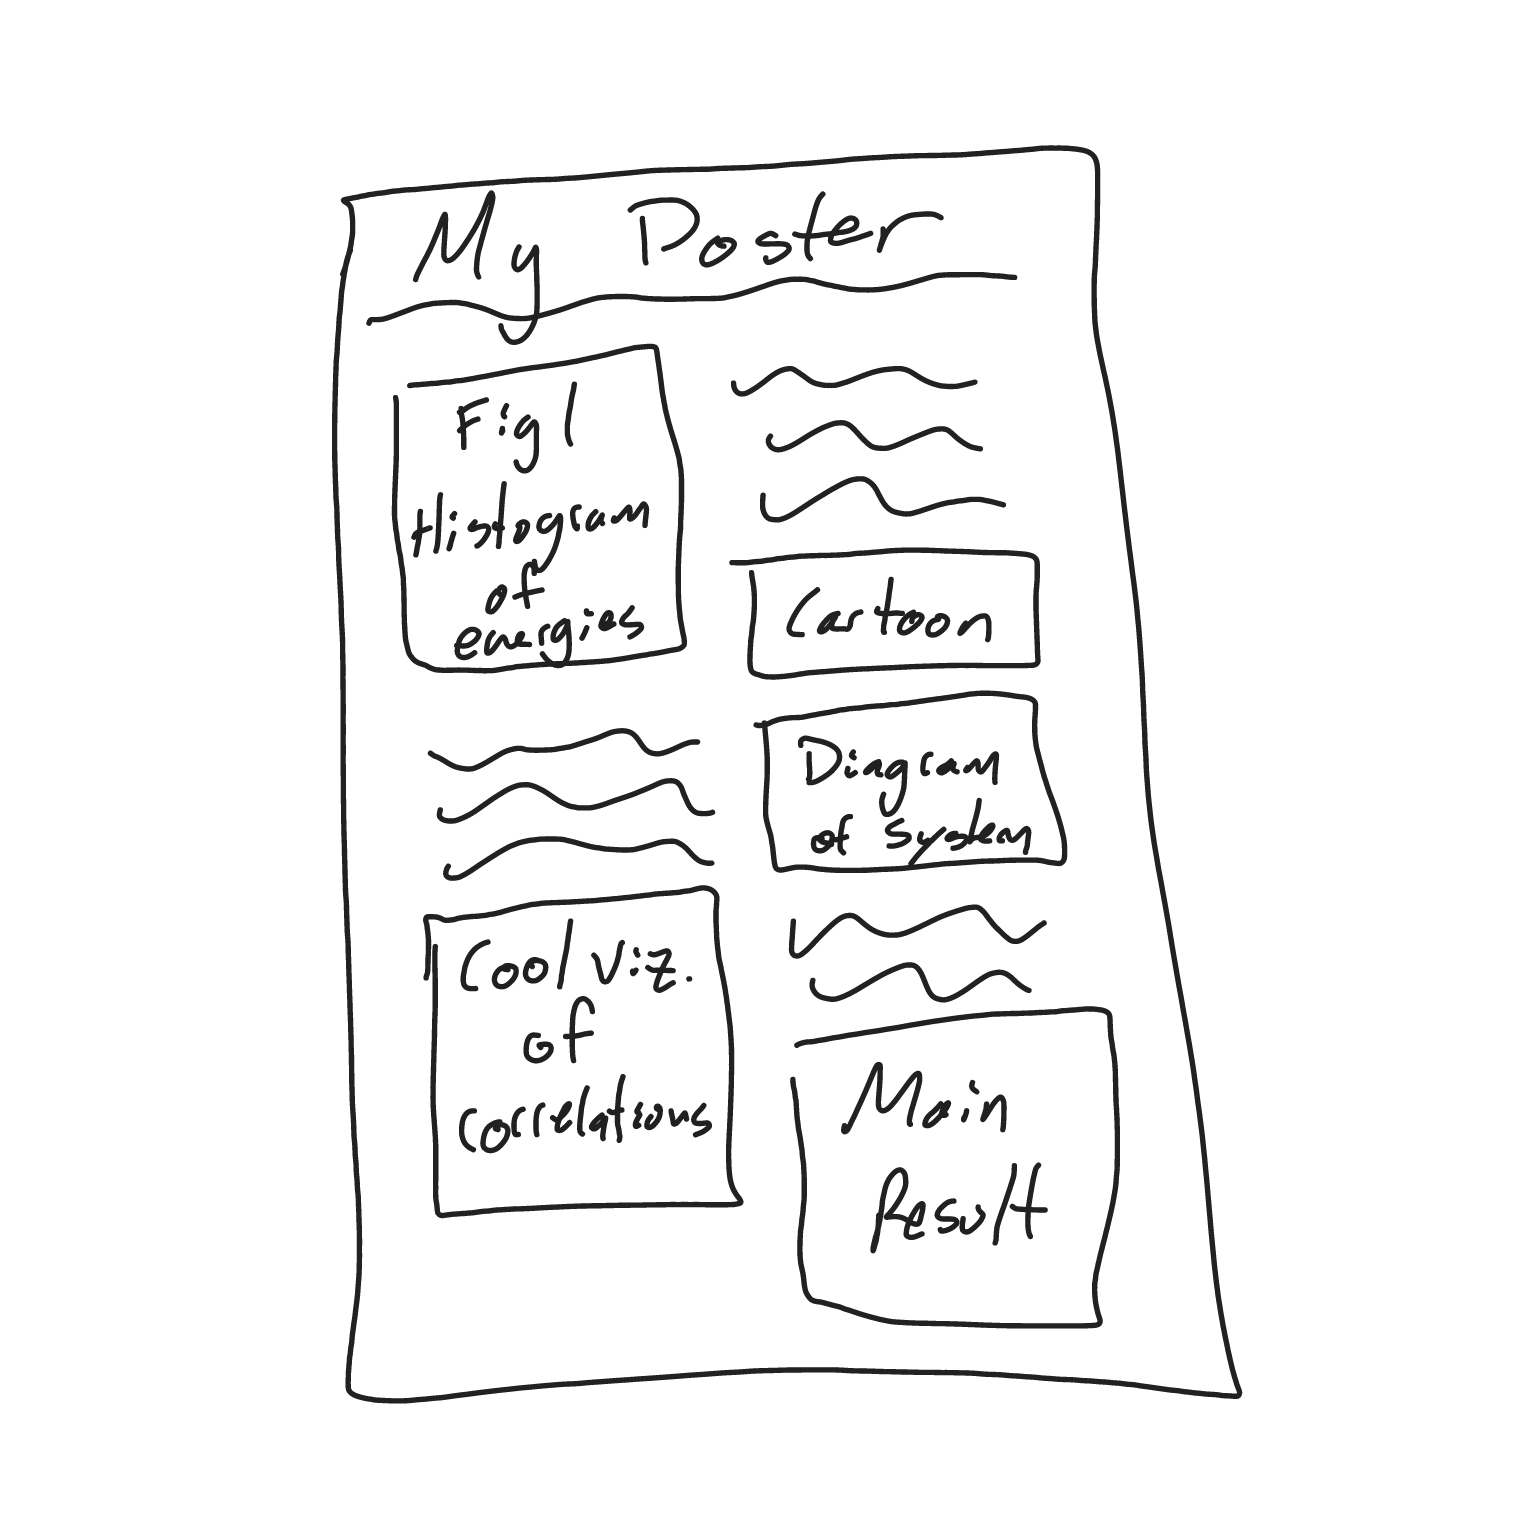
\includegraphics[width=0.9\columnwidth]{../Lecture3/PosterConcept.png}\\
    \includegraphics[width=0.6\columnwidth]{/Users/fizisist/Documents/UChicago/Teaching/ComputationalPhysics/PHYS250/PHYS250-Autumn2024/FinalProjects/FinalPosterComputationalPhysics.pdf}\\
  \end{figure}

  
  \end{columns}

  
\end{frame}

%-----------------------------------------------------------------------------------------

\begin{frame}%[shrink=10]
  \frametitle{Poster project example}
  
  \begin{figure}
    \includegraphics[width=0.90\columnwidth]{/Users/fizisist/Documents/UChicago/Teaching/ComputationalPhysics/PHYS250/PHYS250-Autumn2024/FinalProjects/FinalPosterComputationalPhysics.pdf}
  \end{figure}
  
\end{frame}

%==========================================================================================
\section[Introduction to minimization]{Introduction to minimization}
%==========================================================================================

%-----------------------------------------------------------------------------------------
\subsection[Minimization is everywhere]{Minimization is everywhere}
%-----------------------------------------------------------------------------------------

\begin{frame}%[shrink=10]
  \frametitle{Minimization is everywhere}

  As physicists, we are \bluebf{constantly attempting to minimize or maximize functions that describe the world around us}.
  
  \vspace{0.3cm}
  
  \begin{ucblock}{Examples of minimization}
    \begin{itemize}
      \item \bluebf{Fitting a model to data:} minimize differences between a model and data
      \item \bluebf{Second law of thermodynamics:} minimize changes in entropy for a system in thermodynamic equilibrium
      \item \bluebf{Conservation of momentum:} establish mechanical equilibrium by minimizing changes in momentum, $\frac{d\vec{p}}{dt}=0$
      \item \bluebf{Principle of least action:} obtain the equations of motion of a system by minimizing (or maximizing!) the variations of the action, $S$
      \item \bluebf{Path integral formulation of quantum mechanics:} sort quantum mechanically possible trajectories by minimizing quantum action
      \item \bluebf{Ising model:} minimization the energy of the spin configurations
    \end{itemize}
  \end{ucblock}

\end{frame}



%-----------------------------------------------------------------------------------------

\begin{frame}%[shrink=10]
  \frametitle{Energy Minimization from your first year text books}

  \begin{figure}
    \centering
    \includegraphics[width=\textwidth]{MinimaMaximaEnergy.pdf}
  \end{figure}

\end{frame}

%-----------------------------------------------------------------------------------------

\begin{frame}%[shrink=10]
  \frametitle{Minimization can imply maximization \ra\ optimization}

  \begin{figure}
    \centering
    \includegraphics<1>[width=\textwidth,angle=0]{PotentialEnergy.pdf}
    \includegraphics<2>[width=\textwidth,angle=180]{PotentialEnergy.pdf}
  \end{figure}

\end{frame}

%-----------------------------------------------------------------------------------------
\subsection[Statement of the problem]{Statement of the problem}
%-----------------------------------------------------------------------------------------

\begin{frame}%[shrink=10]
  \frametitle{Optimization, or finding the extrema of a system}

  Since we are most often interested in maxima or minima of the evolution or behavior of a system as a function of some external parameter, the problem often boils down to the determination of \bluebf{first and second derivatives} as a function of that parameter.
  
  \begin{equation}
    f(x) \approx f(a)+{\frac {f'(a)}{1!}}(x-a)+{\frac {f''(a)}{2!}}(x-a)^{2}+{\frac {f'''(a)}{3!}}(x-a)^{3}+\cdots ,
  \end{equation}
  
  If we focus only on the first three terms, we can write this for a function of $n$ variables $\vec{x} = \sum_{i=0}^{n}x_i$ as:
  
  \begin{equation}
    f(\vec{x}) \approx f(\vec {a} )+ (\vec{x} - \vec{a})^{\mathrm {T} }  \nabla f(\vec{a}) +{\frac {1}{2!}}(\vec{x} - \vec{a})^{\mathrm {T} }\mathbf {H} (\vec{a})(\vec{x} - \vec{a})
  \end{equation}
  
  where $\mathbf {H}$ is the \bluebf{Hessian matrix}, describing the \alertbf{curvature} of $f(\vec{x})$ by

  \begin{equation}
    {\mathbf {H} }_{i,j}={\frac {\partial ^{2}f(\vec{a})}{\partial x_{i}\partial x_{j}}}
  \end{equation}
  
  (Note: The determinant of $\mathbf {H}$ is also sometimes referred to as \alertbf{the Hessian}.)
  
\end{frame}

%-----------------------------------------------------------------------------------------

\begin{frame}%[shrink=10]
  \frametitle{Optimization methods and approaches}

  There are many details associated with the \alertbf{existence, feasibility, and constraints} on the optimization problem for finding and describing extrema.
  
  \vspace{0.3cm}
  
  Assuming that these are generally satisfied, we can categorize the approaches into two primary groups and specific implementations of each:
  
  \begin{itemize}
    \item \bluebf{Evaluate second derivatives (Hessians):} Newton's method is the most famous and widely used
    \item \bluebf{Evaluate first derivatives (gradients):} Gradient descent is perhaps the most widely used 
  \end{itemize}
  
  Then, there is a kind of ``hybrid'' approach which is referred to as \bluebf{quasi-Newton} wherein the Hessian matrix is approximated using updates specified by gradient evaluations.
  
  \vspace{0.3cm}
  
  We will come back to these methods on Thursday, but for now, let's discuss a simple minimization: \alertbf{Least squares}
  
\end{frame}

%==========================================================================================
\section[Least squares minimization]{Least squares minimization}
%==========================================================================================

%-----------------------------------------------------------------------------------------
\subsection[Linear regression]{Linear regression}
%-----------------------------------------------------------------------------------------

\begin{frame}%[shrink=10]
  \frametitle{Linear regression (II)}

  Suppose that you want to fit a set data points $(x_i,y_i)$, where $i = 1,2,\ldots,N$, to a straight line, $y=ax+b$.
  
  \begin{figure}
    \centering
    \includegraphics<1>[width=0.5\textwidth,angle=0]{../../Examples/Normal_vs_ODR.png}
  \end{figure}
  
  The process of determining the best-fit line is called \alertbf{linear regression}.  This involves choosing the parameters $a$ and $b$ to minimize the sum of the squares of the differences between the data points and the linear function.
  
\end{frame}

%-----------------------------------------------------------------------------------------

\begin{frame}%[shrink=10]
  \frametitle{Linear regression (II)}

  Suppose that you want to fit a set data points $(x_i,y_i)$, where $i = 1,2,\ldots,N$, to a straight line, $y=ax+b$.
  
  \begin{figure}
    \centering
    \includegraphics<1>[width=0.5\textwidth,angle=0]{../../Examples/Normal_vs_ODR.png}
  \end{figure}
  
  If there are only uncertainties in the $y$ direction, then the differences in the vertical direction (the gray lines in the figure) are used.  If there are uncertainties in both the $x$ and $y$ directions, the orthogonal (perpendicular) distances from the line (the dotted red lines in the figure) are used.
  
\end{frame}

%-----------------------------------------------------------------------------------------
\subsection[Curve fitting]{Curve fitting}
%-----------------------------------------------------------------------------------------


\begin{frame}%[shrink=10]
  \frametitle{Using the $\chi^2$ (again!)}

  For the case where there are only uncertainties in the $y$ direction, there is an analytical solution to the problem.  
  
  \vspace{0.3cm}
  
  If the uncertainty in $y_i$ is $\sigma_i$, then the difference squared for each point is weighted by $w_i=1/\sigma_i^2$. The function to be minimized with respect to variations in the parameters, $a$ and $b$, is  

  \begin{equation}
    \chi^2 = \sum_{i=1}^N w_i \left[y_i - \left(ax_i+b\right)\right]^2.
  \end{equation}
    
The analytical solutions for the best-fit parameters that minimize $\chi^2$ are those that satisfy $\frac{\partial (\chi^2)}{\partial a}=0$ (and similarly for $b$).
  
\end{frame}

%-----------------------------------------------------------------------------------------


\begin{frame}%[shrink=10]
  \frametitle{Uncertainties}

  From the above equation for the $\chi^2$, we can obtain $a$ and $b$ from:

  \begin{equation}
    a=\frac{\sum w_i \sum w_i x_i y_i - \sum w_i x_i \sum w_i y_i}{\sum w_i \sum w_i x_i^2 - \left(\sum w_i \sum w_i x_i\right)^2}
  \end{equation}

  and
  
  \begin{equation}
    b=\frac{\sum w_i y_i \sum w_i x_i^2 - \sum w_i x_i \sum w_i x_i y_i}{\sum w_i \sum w_i x_i^2 - \left(\sum w_i \sum w_i x_i\right)^2}.
  \end{equation}
  
  The uncertainties in the parameters are  

  \begin{eqnarray}
    \sigma_a &=& \sqrt{\frac{\sum w_i}{\sum w_i \sum w_i x_i^2 - \left(\sum w_i \sum w_i x_i\right)^2}} \\
    \sigma_b &=& \sqrt{\frac{\sum w_i x_i^2}{\sum w_i \sum w_i x_i^2 - \left(\sum w_i \sum w_i x_i\right)^2}}.
  \end{eqnarray}
  
All of the sums in the four previous equations are over $i$ from 1 to $N$.  
  
\end{frame}

%
%For a $30\times30$ lattice with 20,000 time steps per simulation, I was seeing 2.5s/simulation or about 2-3 min to run 100 simulations at different temperatures

%%==========================================================================================
%\section[Conclusions]{Conclusions}
%==========================================================================================
%
%\begin{frame}%[shrink=1]
%  \frametitle{Conclusions}
%
%  \begin{itemize}
%    \item Something
%  \end{itemize}
%  
%\end{frame}

%==========================================================================================
%==========================================================================================
\end{document}
